 \documentclass[twoside,12pt]{article}

\usepackage{../dsctemplate}
\usepackage[margin=1in]{geometry}
\usepackage{amsmath}
\usepackage{amssymb,amsthm}
\usepackage{fancyhdr}
\usepackage{nicefrac}
\usepackage{minted, latex2pydata}
\usetikzlibrary{quotes,angles,positioning,arrows.meta}
\usetikzlibrary{calc}
\usepackage{enumitem}
\usepackage{fancyvrb}
\usepackage{dirtytalk}
\usepackage{comment}
\usepackage{graphicx}
\usepackage{setspace}

\usepackage{amsmath,amssymb,amsfonts,amsthm}

\usepackage{booktabs}
\usepackage{pgfplots}
\usepackage{url}
\usepackage{scrextend}
\usepackage{multido}
\usepackage{graphbox}
\usepackage{pdfpages}
\usepackage{gensymb}
\usepackage{hhline}
\usepackage{multicol}
\DefineVerbatimEnvironment{verbatim}{Verbatim}{xleftmargin=.5in}
\newlist{multiplechoice}{itemize}{2}
\setlist[multiplechoice]{label=$\square$}

% configuration
% ------------------------------------------------------------------------------

% control whether solutions are shown or hidden
%\showsolntrue

% page headers only on odd pages
\pagestyle{fancy}
\fancyhead{}
\fancyhead[RO]{PID: \rule{3in}{.5pt}}
\renewcommand{\headrulewidth}{0pt}
% \pagenumbering{gobble}

\usepackage{xcolor, soul}
\newcommand{\hlc}[2][yellow]{{%
		\colorlet{foo}{#1}%
		\sethlcolor{foo}\hl{#2}}%
}

\newcommand{\sawyer}[1] {{ \textcolor{blue}{\hlc[blue!15]{\sf [SJR:] #1}}}}
\newcommand{\attn}[1] {{ \textcolor{black}{\hlc[yellow!75]{\sf #1}}}}

\newcommand{\pr}[1]{\mathbb{P}\left[{#1}\right]}

\newcommand{\python}[1]{\mintinline{python}{#1}}
\newcommand{\yes}{Yes}
\newcommand{\given}{\,|\,}


\usepackage{multido}
\usetikzlibrary{positioning}

\newcommand{\avocado}{%
  \begingroup\normalfont
  \includegraphics[height=2\fontcharht\font`\B, align=c]{pics/avo.png}%
  \endgroup
}

\newcommand{\avo}[1]{\multido{}{#1}{\avocado}\hspace{0.2em}}

% ------------------------------------------------------------------------------
\showsolntrue
%\showsolnfalse

\begin{document}

\thispagestyle{empty}

\vspace{-5.5in}

\pstitle{%
	Final Exam
	}{DSC 40A, Fall 2024}

\vspace{-.3in}

\begin{tabular}{rl}
	Full Name:   & \inlineresponsebox[4in]{Solutions} \\
	PID:         & \inlineresponsebox[4in]{A12345678} \\
	Seat Number: & \inlineresponsebox[4in]{A1}        
	% Lecture: & \bubble{A (10AM)} \bubble{B (9AM)} \bubble{C (1PM)} \bubble{D (8AM)} \vspace{.3in} \\ 
\end{tabular}

\vspace{.1in}

\vspace{.1in}


\textbf{Instructions:}
\begin{itemize}
	\item This exam consists of 9 questions, worth a total of 100 points. 
	      \textbf{All questions on the exam count towards your Final Exam score, but Questions 1-4 count towards your Midterm Redemption score.}
	              
	\item \textbf{Advice: Read all of the questions before starting to work, because the questions are not sorted by difficulty.}
	\item Write your PID in the top right corner of each page in the space provided.
	\item Please write \textbf{clearly} in the provided answer boxes; we will not grade work that appears elsewhere.
	      \begin{itemize}
	      	\item For questions that ask you to show your work, correct answers with no work shown will receive no credit.
	      	      %\item When asked to do so, please place your final answer in a $\boxed{\text{box}}$.
	      	      %\item \bubble{In multiple choice questions, select only one option and completely fill in the corresponding bubble --- if we cannot tell which option you selected, you may not receive credit.}
	      \end{itemize}
	\item {You may use two pages two-sided as a cheat sheet. Other than that, you may not refer to any resources or technology during the exam (no phones, no smart watches, no computers, and no calculators).}
\end{itemize}

\vspace{.1in}

\vspace{.2in}

\noindent By signing below, you are agreeing that you will behave honestly and fairly during
and after this exam. 

\begin{tabular}{rl}
	\: \: \: \: \: Signature: & \inlineresponsebox[4in]{} \\
\end{tabular}

\vfill

\begin{center}
	{\huge Version A} \vspace{.2in}
	
	Please do not open your exam until instructed to do so.
	
\end{center}

\newpage

\begin{probset}
	
	\begin{prob}[(10 points)] %Empirical risk minimization 
		
		For each statement below, fill in the circle indicating the word(s) or phrase(s) which would make the statement correct if added to the sentence. In several statements, $(y_i)_{i=1}^n$ denotes a dataset of real numbers. \textit{You do not need to show your work for full credit, but partial credit may be awarded for supporting calculations and reasoning.}
		
		% \begin{subprob}
		%     If $x^\ast$ is a minimizer for $f(x)$ and $f(x)\geq 0$ for all $x$, then $x^\ast$ is a \rule{1in}{.15mm} for $\sqrt{f(x)}$.    
		% \end{subprob}
		
		% \begin{responsebox}{1in}
		%     The correct answer is \textbf{minimizer}. If $x^\ast$ is a minimizer for $f$, then $f(x^\ast)\leq f(x)$ for all $x$, so $\sqrt{f(x)}\leq\sqrt{f(x^\ast)}$ for all $x$, so $x^\ast$ is a minimizer for $\sqrt{f}$.
		% \end{responsebox}
		
		\begin{subprob}\avo{2}
			If $x^\ast$ is a maximizer for $f(x)$ and $f(x)\geq 0$ for all $x$, then $x^\ast$ is a \rule{1in}{.15mm} for $g(x)=3-f(x)^2$.  
			\vspace*{-.125in}
			\begin{center}
				\begin{tabular}{ccc}
					$\bigcirc$ minimizer & \hspace{.25in}$\bigcirc$ maximizer & \hspace{.25in}$\bigcirc$ neither 
				\end{tabular}
			\end{center}
		\end{subprob}
		
		\begin{responsebox}{1.25in}
			The correct answer is \textbf{minimizer}. Note that $g(x) = 3-f(x)^2$ is a monotone decreasing function for $x\geq 0$. Therefore, since $f(x) \leq f(x^\ast)$ for all $x$, $g(f(x)) \geq g(f(x^\ast))$ for all $x$ and this $x^\ast$ is a minimizer for $3-f^2$.
		\end{responsebox}
		
		% \begin{subprob}
		%     Let $ (y_i)_{i=1}^n = (y_1,\dotsc, y_n)\in\mathbb{R}$. Then the minimizer of the empirical risk of the absolute loss\\ \\function for a constant prediction of $(y_i)_{i=1}^n$ is the \rule{1in}{.15mm} of $(y_i)_{i=1}^n$.
		% \end{subprob}
		
		% \begin{responsebox}{1in}
		%     The correct answer is \textbf{median}. See lecture 4 notes.
		% \end{responsebox}
		
		% \begin{subprob}
		%     Let $ (y_i)_{i=1}^n = (y_1,\dotsc, y_n)\in\mathbb{R}$. Then the squared loss for a constant prediction of $(y_i)_{i=1}^n$ is \\ \\\rule{1in}{.15mm} robust to outliers when compared to the absolute loss.
		% \end{subprob} 
		    
		% \begin{responsebox}{1in}
		%     The correct answer is \textbf{less} robust. See lecture 4 notes.
		% \end{responsebox}
		
		\begin{subprob}\avo{2}
			Suppose we wish to find a constant predictor for $y$ using either squared or absolute loss. In high-stakes scenarios where outliers are rare but of great importance, it is better to use the \rule{1in}{.15mm} function.
			\vspace*{-.125in}
			\begin{center}
				\begin{tabular}{cc}
					$\bigcirc$ absolute loss & \hspace{.25in}$\bigcirc$ squared loss 
				\end{tabular}
			\end{center}
			
		\end{subprob}
		
		\begin{responsebox}{1in}
			The answer is \textbf{squared} loss, since it is more sensitive to outliers.
		\end{responsebox}
		
		\begin{subprob}\avo{2}
			Let $(1, 3, 4, 1, 2, -1)$ be a dataset of real numbers. The derivative of the empirical risk for the absolute loss $L_{abs}(h)$ of a constant predictor $h$ for the datset is \rule{1in}{.15mm} when $h=2.5$.
			\vspace*{-.125in}
			\begin{center}
				\begin{tabular}{ccc}
					$\bigcirc$ positive & \hspace{.25in}$\bigcirc$ negative & \hspace{.25in}$\bigcirc$ zero 
				\end{tabular}
			\end{center}
			
		\end{subprob}
		
		\begin{responsebox}{1.25in}
			The derivative of empirical risk for absolute loss is given by
			\[R'(h) = \frac{1}{n}\sum_{i=1}^n\mathrm{sign}(h - y_i).\]
			See lectures 3-4 for a derivation. Thus
			\[R'(2.5) = \frac{1}{6}(1 -1 -1 +1 +1 +1) = \frac{1}{3} > 0 .\]
			So the correct answer is \textbf{positive}.
			
			Alternative solution. 
			Order the daatset: $(-1,1, 1, 2, 3, 4 )$.
			The loss is minimized in the range [1,2].
			The point $h=2.5$ is to the right of this minimum and therefore the function is increasing at this point and the derivative must be positive. 
			
		\end{responsebox}
		
		\newpage
		\begin{subprob}\avo{2}
			Assume a dataset $\{y_i\}_{i=1}^n$ satisfies $y_i\in[0,1]$ for all $i$. Let $h^\ast$ denote the optimal constant predictor for the dataset with respect to squared loss. Assume we sample a new data point $y_{n+1}$ where $y_{n+1}=y_4 - 2$. Then the new minimizer $h'$ is \rule{1in}{.15mm} the old minimizer $h^\ast$.
			    
			\vspace*{-.125in}
			\begin{center}
				\begin{tabular}{ccc}
					$\bigcirc$ greater than & \hspace{.25in}$\bigcirc$ less than & \hspace{.25in}$\bigcirc$ equal to 
				\end{tabular}
			\end{center}
		\end{subprob}
		
		
		\begin{responsebox}{1.5in}
			We have that $h^\ast$ is the mean of the original data, and $h'$ is the mean of the new data. Therefore
			\begin{align}
				h' & = \frac{1}{n+1}\sum_{i=1}^{n}y_i = \frac{1}{n+1}(y_1+\cdots+y_n + (y_4 - 2)) \\
				   & = \frac{1}{n+1}(n h^\ast + (y_4 - 2))                                        \\
				   & = \frac{n}{n+1}h^\ast + \frac{y_4 - 2}{n+1}                                  
			\end{align}
			Note that $y_4 - 2 \leq 1 - 2 = -1 < 0$, so that 
			\begin{align}
				\frac{n}{n+1}h^\ast + \frac{y_4 - 2}{n+1} < \frac{n}{n+1}h^\ast < h^\ast 
			\end{align}
			Therefore the correct answer is \textbf{less than}.
		\end{responsebox}
		
		\begin{subprob}\avo{2}
			Let $\epsilon > 0$ be any positive real number. Define the smooth loss by the formula
			\[L_{\epsilon}(h, y_i) = \sqrt{|y_i - h|^2+ \epsilon^2}.\]
			Then the optimal \textit{value} of the empirical risk of $L_{\epsilon}$ is  \rule{1in}{.15mm} the optimal \textit{value} of the empirical risk of the absolute loss function.
			    
			\vspace*{-.125in}
			\begin{center}
				\begin{tabular}{ccc}
					$\bigcirc$ greater than & \hspace{.25in}$\bigcirc$ less than & \hspace{.25in}$\bigcirc$ equal to 
				\end{tabular}
			\end{center}
		\end{subprob}
		
		\begin{responsebox}{1.5in}
			Note that
			\[L_{\epsilon}(h, y_i) = \sqrt{|y_i - h|^2+ \epsilon^2} >\sqrt{|y_i - h|^2} = |y_i-h| = L_{abs}(h, y_i).\]
			Therefore the minimum value of $L_{\epsilon}$ is \textbf{greater} than the minimum value of $L_{abs}$.
		\end{responsebox}
		
		
	\end{prob}
	%\begin{subprob}
	%   For $n=1, 2, \dotsc$ let $h^\ast_n$ be any minimizer of the empirical risk for the loss
	%      \[L_p(h, y_i) = |y_i - h|^n\]
	%   Then $h^\ast = \lim_{p\rightarrow\infty} h^\ast_p$ exists and is equal to the \rule{1in}{.15mm} \{mean, median, midrange, mode\} of $(y_i)_{i=1}^n$.
	%\end{subprob}
	
	%\begin{responsebox}{1in}
	%   The answer is \textbf{midrange}, see Lecture 4 notes.
	%\end{responsebox}
	
\end{probset}

\newpage

\begin{probset}
	\begin{prob}[(12 points)] %Empirical Risk Minimization 
		Suppose you are designing a central temperature control system for a network of $n\geq 1$ houses in a small town. Each house \( i \) has a preferred temperature \( y_i \), and the importance of satisfying house \( i \)'s preference is represented by a weight \( a_i > 0 \), which represents the number of residents in each house.
		        
		The system is set to maintain a single uniform temperature \( h \) across all houses. To minimize dissatisfaction, you aim to minimize the weighted squared error:
		        
		\[
			R(h) = \frac{1}{n}\sum_{i=1}^n a_i (y_i - h)^2.
		\]
		
		\begin{subprob}\avo{4}
			Find a formula for the optimal temperature $h^\ast$ in terms of the various preferred temperatures $y_1,\dotsc, y_n$. \textit{Show all your calculations.}
		\end{subprob}
		    
		\begin{responsebox}{2in}            
			To minimize the function \( R(h) = \sum_{i=1}^n a_i (y_i - h)^2 \), we differentiate \( R(h) \) with respect to \( h \) and set the derivative equal to zero:
			\[
				\frac{dR(h)}{dh} = \frac{d}{dh} \sum_{i=1}^n a_i (y_i - h)^2 = -2 \sum_{i=1}^n a_i (y_i - h).
			\]
			Setting \( \frac{dR(h)}{dh} = 0 \), we get:
			\[
				\sum_{i=1}^n a_i y_i - \sum_{i=1}^n a_i h = 0.
			\]
			Simplifying:
			\[
				h \sum_{i=1}^n a_i = \sum_{i=1}^n a_i y_i.
			\]
			Solving for \( h^\ast \):
			\[
				h^\ast = \frac{\sum_{i=1}^n a_i y_i}{\sum_{i=1}^n a_i}.
			\]
			Thus, the optimal temperature \( h^\ast \) is the weighted average of the preferred temperatures.
		\end{responsebox}
		
		\begin{subprob}\avo{3}
			Suppose that the family which lives in house $1$ has a baby, and their weight $a_1$ increases by one. Assuming their preferred temperature does not change, find an expression which relates the \emph{new} optimal temperature $h'$ to the old optimal temperature $h^\ast$ you found in (a). \textit{Show all your calculations.}
		\end{subprob}
		
		\begin{responsebox}{2in} Let \( h' \) denote the new optimal temperature. The new weight for house \( 1 \) becomes \( a_1' = a_1 + 1 \). Using the formula for \( h^\ast \), the new optimal temperature is:
			\[
				h' = \frac{(a_1 + 1)y_1 + \sum_{i=2}^n a_i y_i}{(a_1 + 1) + \sum_{i=2}^n a_i}.
			\]
			Expanding \( h' \):
			\[
				h' = \frac{a_1 y_1 + y_1 + \sum_{i=2}^n a_i y_i}{a_1 + 1 + \sum_{i=2}^n a_i}= \frac{ y_1 + \sum_{i=1}^n a_i y_i}{  1 + \sum_{i=1}^n a_i}.
			\]
			Factoring out the original terms for \( h^\ast \):
			\[
				h' = \frac{h^\ast \sum_{i=1}^n a_i + y_1}{\sum_{i=1}^n a_i + 1}.
			\]
			This relates the new optimal temperature \( h' \) to the original \( h^\ast \) by accounting for the additional weight and the corresponding preference.
		\end{responsebox}
		
		%\newpage
		\begin{subprob}\avo{5}
			You and your colleagues are discussing new and improved ways to set the weights used in the cost function. Your team comes up with three alternatives for setting the weights:
			\begin{itemize}
				\item $a_i = (\text{the number of residents in house $i$})$, 
				\item $b_i = 1$ for all houses,
				\item $c_i = 1/(\text{the number of windows in house $i$})$.
			\end{itemize}
			Assume each house is occupied by at least one person and has at least one window. Let 
			\begin{itemize}
				\item $A$ denote the optimal risk of $R(h)$ with respect to the weights $a_i$
				\item $B$ denote the optimal risk of $R(h)$ with respect to the weights $b_i$
				\item $C$ denote the optimal risk of $R(h)$ with respect to the weights $c_i$
			\end{itemize}
			\textbf{Using the relations} $<,\leq,>,\geq,=$, rank the numbers $A,B,C$ from least to greatest. \textit{Explain your reasoning and don't forget about the baby!}
		\end{subprob}
		
		\begin{responsebox}{3in}  Note that for any choice of $h$, we have the following inequalities:
			\[
				\sum_{i=1}^n c_i (y_i - h)^2\leq \sum_{i=1}^n b_i (y_i - h)^2 <\sum_{i=1}^n a_i (y_i - h)^2.
			\]
			since $c_i \leq 1$ for all $i$, $b_i = 1$ for all $i$, and $a_i\geq 1$ for all $i$. Therefore the minimum values for each such function with respect to $h$ will follow these inequalities. That is,
			\[
				C\leq B < A.
			\]

            (Note we also accepted solution $C\leq B \leq A$ for those who forgot about the baby ;) )
		\end{responsebox}
	\end{prob}
	    
\end{probset}

\newpage


\begin{probset}
	\begin{prob}[(10 points)] %Linear regression
		    
		A local farmers' market vendor sells homemade jam jars and is analyzing the relationship between the number of hours she spends at the market and the number of jam jars sold. Over three weekends, she collects the following data:
		
		\begin{itemize}
			\item \textbf{Weekend 1}: Worked for 1 hour, sold 2 jars.
			\item \textbf{Weekend 2}: Worked for 2 hours, sold 4 jars.
			\item \textbf{Weekend 3}: Worked for 3 hours, sold 6 jars.
		\end{itemize}
		    
		Noticing a perfect linear trend, she decides to model this relationship using linear regression. Let $x_1 = 1, x_2=2, x_3=3$ denote the number of hours she worked on the corresponding weekend and let $y_1 = 2, y_2=4, y_3=6$ denote the number of jars sold.
		
		\begin{subprob}\avo{2}
			First, fill in the blanks in the table below which gathers relevant information for least squares regression. Then, find the optimal parameters $w_0^\ast$ and $w_1^\ast$ for a simple least squares linear model for her jar sales. \textit{Show all your calculations.}
		\end{subprob}
		    
		\begin{center}
			\begin{tabular}{|c|c|}\hline
				$\sum_{i=1}^3 x_i$    & 6               \\ [.25cm] \hline
				$\sum_{i=1}^3 y_i$    & \rule{2cm}{0pt} \\ [.25cm] \hline
				$\sum_{i=1}^3 x_iy_i$ & 28              \\ [.25cm] \hline
				$\sum_{i=1}^3 x_i^2$  &                 \\ [.25cm]\hline
			\end{tabular}
		\end{center}
		
		\begin{responsebox}{3.2in}
		\begin{center}
			\begin{tabular}{|c|c|}\hline
				$\sum_{i=1}^3 x_i$    & 6               \\ [.25cm] \hline
				$\sum_{i=1}^3 y_i$    & 12 \\ [.25cm] \hline
				$\sum_{i=1}^3 x_iy_i$ & 28              \\ [.25cm] \hline
				$\sum_{i=1}^3 x_i^2$  & 14 \\ [.25cm]\hline
			\end{tabular}
		\end{center}
        
			To calculate the optimal parameters:
			
			\[
			w_1^\ast = \frac{\sum_{i=1}^3 x_i y_i - \frac{1}{3} \sum_{i=1}^3 x_i \sum_{i=1}^3 y_i}{\sum_{i=1}^3 x_i^2 - \frac{1}{3} \left( \sum_{i=1}^3 x_i \right)^2}
			\]
			Substituting values:
			\[
			w_1^\ast = \frac{28 - \frac{1}{3}(6 \cdot 12)}{14 - \frac{1}{3}(6^2)} = \frac{28 - 24}{14 - 12} = \frac{4}{2} = 2
			\]
			
			\[
			w_0^\ast = \frac{1}{3} \sum_{i=1}^3 y_i - w_1^\ast \cdot \frac{1}{3} \sum_{i=1}^3 x_i
			\]
			Substituting values:
			\[
			w_0^\ast = \frac{12}{3} - 2 \cdot \frac{6}{3} = 4 - 4 = 0
			\]
			
			Thus, the optimal parameters are:
			\[
			w_0^\ast = 0, \quad w_1^\ast = 2
			\]

        \end{responsebox}
%		\newpage
		    
		\begin{subprob}\avo{2}
			On a fourth weekend, due to a festival, she couldn't set up her stall but managed to sell 2 jars to early customers who contacted her directly. This data point is:
			\begin{itemize}
				\item \textbf{Weekend 4}: Worked for 0 hours, sold 2 jars.
			\end{itemize}
			She now wants to understand how this outlier affects her overall analysis. Fill out the table below based on the new data point $x_4 = 0, y_4=2$ and then find the \textbf{new} optimal parameters $w_0'$ and $w_1'$ for a simple least squares linear model. \textit{Show all your calculations.}
		\end{subprob}
		
		\begin{center}
			\begin{tabular}{|c|c|}\hline
				$\sum_{i=1}^4 x_i$    & \rule{2cm}{0pt} \\ [.25cm] \hline
				$\sum_{i=1}^4 y_i$    & 14              \\ [.25cm] \hline
				$\sum_{i=1}^4 x_iy_i$ & 28              \\ [.25cm] \hline
				$\sum_{i=1}^4 x_i^2$  &                 \\ [.25cm]\hline
			\end{tabular}
		\end{center}
		
		\begin{responsebox}{2.25in}
			
		\begin{center}
			\begin{tabular}{|c|c|}\hline
				$\sum_{i=1}^4 x_i$    & 6 \\ [.25cm] \hline
				$\sum_{i=1}^4 y_i$    & 14              \\ [.25cm] \hline
				$\sum_{i=1}^4 x_iy_i$ & 28              \\ [.25cm] \hline
				$\sum_{i=1}^4 x_i^2$  & 14 \\ [.25cm]\hline
			\end{tabular}
		\end{center}

            To calculate the new parameters:
			
			\[
			w_1' = \frac{\sum_{i=1}^4 x_i y_i - \frac{1}{4} \sum_{i=1}^4 x_i \sum_{i=1}^4 y_i}{\sum_{i=1}^4 x_i^2 - \frac{1}{4} \left( \sum_{i=1}^4 x_i \right)^2}
			\]
			Substituting values:
			\[
			w_1' = \frac{28 - \frac{1}{4}(6 \cdot 14)}{14 - \frac{1}{4}(6^2)} = \frac{28 - 21}{14 - 9} = \frac{7}{5} = 1.4
			\]
			
			\[
			w_0' = \frac{1}{4} \sum_{i=1}^4 y_i - w_1' \cdot \frac{1}{4} \sum_{i=1}^4 x_i
			\]
			Substituting values:
			\[
			w_0' = \frac{14}{4} - 1.4 \cdot \frac{6}{4} = 3.5 - 2.1 = 1.4
			\]
			
			Thus, the new parameters are:
			\[
			w_0' = 1.4, \quad w_1' = 1.4
			\]
		\end{responsebox}
        
		
		\begin{subprob}\avo{3}
		On each axis below draw: \textbf{(i)} the scatterplot of the corresponding data, and \textbf{(ii)} the line of best fit you found for the corresponding dataset in the preceding parts.
		\end{subprob}
		
		\begin{center}
			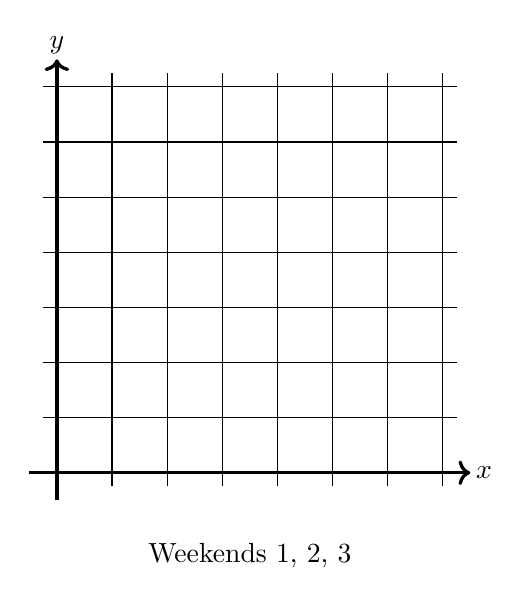
\begin{tikzpicture}[scale=0.7]
				\draw[step=1.0,black,thin] (-0.25,-0.25) grid (7.25, 7.25);
				\draw[->, very thick] (-0.5, 0) -- (7.5,0);
				\node at (7.75, 0) {$x$};
				\draw[->, very thick] (0, -0.5) -- (0,7.5);
				\node at (0, 7.75) {$y$};
				\node at (3.5, -1.5) {\centering Weekends 1, 2, 3};
			\end{tikzpicture}
			\hspace{1in}
			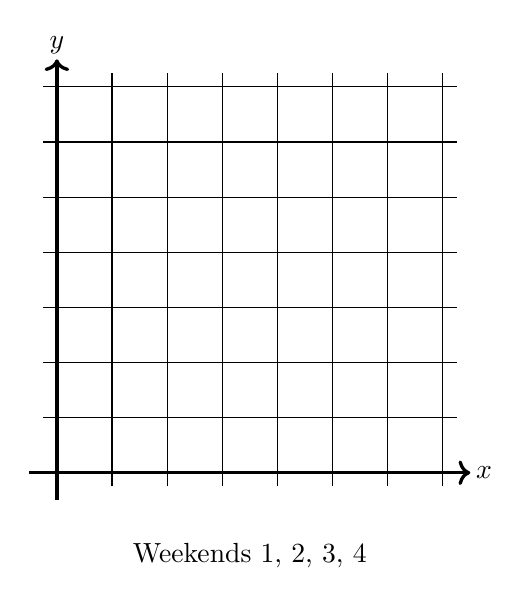
\begin{tikzpicture}[scale=0.7]
				\draw[step=1.0,black,thin] (-0.25,-0.25) grid (7.25, 7.25);
				\draw[->, very thick] (-0.5, 0) -- (7.5,0);
				\node at (7.75, 0) {$x$};
				\draw[->, very thick] (0, -0.5) -- (0,7.5);
				\node at (0, 7.75) {$y$};
				\node at (3.5, -1.5) {\centering Weekends 1, 2, 3, 4};
			\end{tikzpicture}
		\end{center}

		\begin{responsebox}{2in}

        \begin{center}
			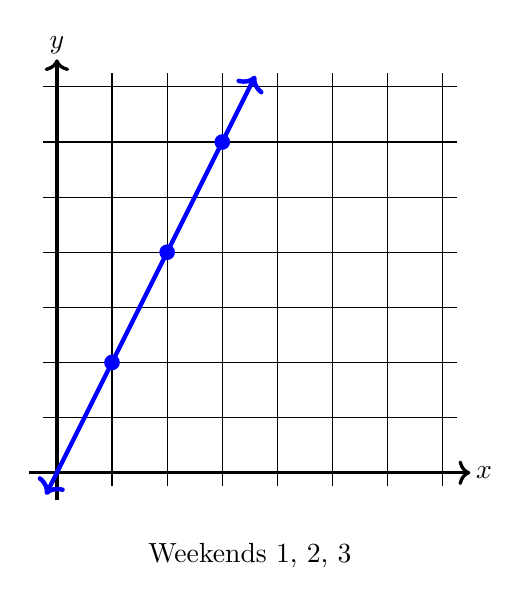
\begin{tikzpicture}[scale=0.7]
				\draw[step=1.0,black,thin] (-0.25,-0.25) grid (7.25, 7.25);
				\draw[->, very thick] (-0.5, 0) -- (7.5,0);
				\node at (7.75, 0) {$x$};
				\draw[->, very thick] (0, -0.5) -- (0,7.5);
				\node at (0, 7.75) {$y$};
				\node at (3.5, -1.5) {\centering Weekends 1, 2, 3};

                \node at (1, 2)[circle,fill,color=blue,inner sep=2pt]{};;
                \node at (2, 4)[circle,fill,color=blue,inner sep=2pt]{};;
                \node at (3, 6)[circle,fill,color=blue,inner sep=2pt]{};;
                \draw[<->, ultra thick, blue] (-.2, -.4) -- (3.6, 7.2);

			\end{tikzpicture}
			\hspace{1in}
			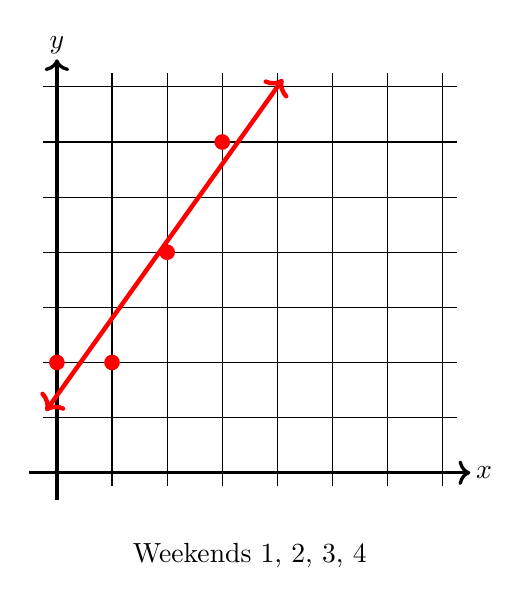
\begin{tikzpicture}[scale=0.7]
				\draw[step=1.0,black,thin] (-0.25,-0.25) grid (7.25, 7.25);
				\draw[->, very thick] (-0.5, 0) -- (7.5,0);
				\node at (7.75, 0) {$x$};
				\draw[->, very thick] (0, -0.5) -- (0,7.5);
				\node at (0, 7.75) {$y$};
				\node at (3.5, -1.5) {\centering Weekends 1, 2, 3, 4};
                
                \node at (0, 2)[circle,fill,color=red,inner sep=2pt]{};;
                \node at (1, 2)[circle,fill,color=red,inner sep=2pt]{};;
                \node at (2, 4)[circle,fill,color=red,inner sep=2pt]{};;
                \node at (3, 6)[circle,fill,color=red,inner sep=2pt]{};;
                \draw[<->, ultra thick, red] (-0.2, 1.12) -- (4.1, 7.14);
			\end{tikzpicture}
		\end{center}
        
        \end{responsebox}

		\begin{subprob}\avo{3}
			Based on the pictures in part \textbf{(c)}, which dataset has greater mean squared error with respect to its optimal parameters? Why? \textit{You do not need to calculate the errors by hand to answer this question. Explain your reasoning.}
		\end{subprob}
		
		\begin{responsebox}{2in}
			The dataset with Weekends 1, 2, 3, and 4 will have a greater mean squared error. This is because the added outlier (Weekend 4) does not follow the original perfect linear trend and introduces a discrepancy between the data points and the new line of best fit.
        \end{responsebox}
		    
		    
	\end{prob}
	
\end{probset}

\newpage

\begin{probset}
	\begin{prob}[(12 points)] %Multiple linear regression 
		
		Consider the usual setup for a multiple regression problem, as follows. Let $\vec{x}_1,\vec{x}_2,\dotsc, \vec{x}_{n}\in\mathbb{R}^d$ be a collection of feature vectors in $\mathbb{R}^d$, and let $X\in\mathbb{R}^{n\times (d+1)}$ be the corresponding design matrix. Each $\vec{x}_i$ has a label $y_i\in\mathbb{R}$, and let $\vec{y}\in\mathbb{R}^n$ be the vector of labels. We wish to fit the data and labels with a linear model
		\[H(\vec{x}) = w_0 + w_1\vec{x}^{(1)} + w_2\vec{x}^{(2)}+\dotsc+ w_d\vec{x}^{(d)} \  = \vec{w}^T\mathrm{Aug}(\vec{x}).\]
		where $\vec{w}\in\mathbb{R}^{d+1}$ is the vector of coefficients with intercept. Let $\vec{w}^\ast$ denote the optimal parameter vector with respect to mean squared error.
		
		For each statement below, fill in the circle indicating the word(s) or phrase(s) which would make the statement correct if added to the sentence. \textit{You do not need to show your work for full credit, but partial credit may be awarded for supporting calculations and reasoning.}
		
		\begin{subprob}\avo{2}
			At $\vec{w}^\ast$, the residual vector $\vec{y}-X\vec{w}^\ast$ is \rule{1.25in}{.15mm} to the column space of the design matrix $X$.
			\vspace*{-.125in}
			\begin{center}
				\begin{tabular}{ccc}
					$\bigcirc$ neither & \hspace{.5in}$\bigcirc$ orthogonal & \hspace{.5in}$\bigcirc$ parallel 
				\end{tabular}
			\end{center}
		\end{subprob}
		\vspace*{-.125in}
		\begin{responsebox}{.8in}
			At $\vec{w}^\ast$, the residual vector $\vec{y} - X\vec{w}^\ast$ is orthogonal to the column space of $X$. This is derived from the normal equations:
			\[
				X^T(\vec{y} - X\vec{w}^\ast) = 0,
			\]
			which imply that the residuals are perpendicular to the space spanned by the columns of $X$.
		\end{responsebox}
		
		\begin{subprob}\avo{2}
			The optimal parameter vector $w^\ast$ is found by setting the \rule{1.25in}{.15mm} of the mean squared error equal to \rule{1.25in}{.15mm} and solving the resulting equation.
			\vspace*{-.125in}
			\begin{center}
				\begin{tabular}{ccc}
					$\bigcirc$ (residuals, $\vec{y}$) & \hspace{.25in}$\bigcirc$ (gradient, the zero vector) & \hspace{.25in}$\bigcirc$ (predicted labels, $X\vec{w}$) 
				\end{tabular}
			\end{center}
		\end{subprob}
		\vspace*{-.125in}
		\begin{responsebox}{.8in}
			The optimal parameter vector $\vec{w}^\ast$ is found by setting the gradient of the mean squared error to the zero vector. The gradient is:
			\[
				\nabla_w \| \vec{y} - X\vec{w} \|^2 = -2X^T(\vec{y} - X\vec{w}),
			\]
			and solving $X^T(X\vec{w} - \vec{y}) = 0$ leads to the normal equation, which gives the minimum.
		\end{responsebox}
		
		\begin{subprob}\avo{2}
			If the features in $X$ are linearly \rule{1.25in}{.15mm}, the matrix $X^TX$ will be \rule{1.25in}{.15mm}, making the normal equation solution possibly undefined.
			\vspace*{-.125in}
			\begin{center}
				\begin{tabular}{ccc}
					$\bigcirc$ (dependent, nonsingular) & \hspace{.25in}$\bigcirc$ (independent, singular) & \hspace{.25in}$\bigcirc$ (dependent, noninvertible) 
				\end{tabular}
			\end{center}
		\end{subprob}
		\vspace*{-.125in}
		\begin{responsebox}{.8in}
			If the features in $X$ are linearly dependent, the matrix $X^TX$ will be singular (noninvertible). Linear dependence implies that the columns of $X$ are not linearly independent, leading to a determinant of zero for $X^TX$, which makes solving the normal equations impossible.
		\end{responsebox}
		
		\begin{subprob}\avo{2}
			If $\vec{c}\in\mathbb{R}^d$ is a fixed vector, and we define $\vec{z}_i' = \vec{x}_i + \vec{c}$, then the \textit{new} optimal parameter vector $\vec{w}'$ for the data $\{\vec{z}_i\}_{i=1}^{n}$ and labels $\vec{y}$ is equal to \rule{1.25in}{.15mm}.
			\vspace*{-.125in}
			\begin{center}
				\begin{tabular}{ccc}
					$\bigcirc$ $\vec{w}^\ast + \mathrm{Aug}(\vec{c})$ & \hspace{.25in}$\bigcirc$ $\vec{w}^\ast$ & \hspace{.25in}$\bigcirc$ $\vec{w}^\ast$ except possibly for $w_0$ 
				\end{tabular}
			\end{center}
		\end{subprob}
		\vspace*{-.125in}
		\begin{responsebox}{1in}
			The new optimal parameter vector $\vec{w}'$ is $\vec{w}^\ast$ except possibly for $w_0$. Adding $\vec{c}$ shifts the features, leaving $w_1, w_2, \dots, w_d$ unchanged but altering the intercept:
			\[
				w_0' = w_0 - \vec{w}^T \vec{c}.
			\]

            (Think of the simple linear regression model - if we shift all the $x_i$'s by constant $c$ this doesn't affect the slope $w_1$ but does affect the intercept $w_0$.)
		\end{responsebox}
		
		For the remaining two parts, fill in the circle which contains the \textbf{gradient} of each function. \textit{You do not need to show your work for full credit, but partial credit may be awarded for supporting calculations and reasoning.}
		
		\begin{subprob}\avo{2}
			Calculate the gradient with respect to $\vec{x}$ of $F(\vec{x}) = \vec{w}^T\mathrm{Aug}(\vec{x})$. 
			            
			\vspace*{-.125in}
			\begin{center}
				\begin{tabular}{ccc}
					$\bigcirc$ $\begin{bmatrix}
					w_1 & w_2 & \dotsc & w_d 
					\end{bmatrix}^T$ &\hspace{.25in}$\bigcirc$ $\vec{x}$ &\hspace{.25in}$\bigcirc$ $\begin{bmatrix}
					w_0 & w_1 & \dotsc & w_d 
					\end{bmatrix}^T$
				\end{tabular}
			\end{center}
		\end{subprob}
		\vspace*{-.125in}
		\begin{responsebox}{1.75in}
			The gradient of $F(\vec{x}) = \vec{w}^T\mathrm{Aug}(\vec{x})$ with respect to $\vec{x}$ is $\begin{bmatrix} w_1 & w_2 & \dotsc & w_d \end{bmatrix}^T$. The first slot in $\mathrm{Aug}(\vec{x})$ is a constant $1$, which cancels out when differentiating.
		\end{responsebox}
		
		\begin{subprob}\avo{2}
			Calculate the gradient with respect to $\vec{w}$ of $F(\vec{w}) = \|\vec{y}-X\vec{w}\|^2$.
			            
			\vspace*{-.125in}
			\begin{center}
				\begin{tabular}{ccc}
					$\bigcirc$ $-2X^TX\vec{w}$ & \hspace{.25in}$\bigcirc$ $-2(\vec{y}-X\vec{w})$ & \hspace{.25in}$\bigcirc$ $-2X^T(\vec{y}-X\vec{w})$ 
				\end{tabular}
			\end{center}
		\end{subprob}
		\vspace*{-.125in}
		\begin{responsebox}{1.75in}
			First expand the squared norm:
			\[
				F(\vec{w}) = (\vec{y} - X\vec{w})^T (\vec{y} - X\vec{w})
			\]
			The gradient of $F(\vec{w})$ with respect to $\vec{w}$ is:
			\[
				\nabla_{\vec{w}} F(\vec{w}) = \nabla_{\vec{w}} \left[ \vec{y}^T\vec{y} - 2\vec{y}^T X\vec{w} + \vec{w}^T X^T X \vec{w} \right]
			\]
			Since $\vec{y}^T\vec{y}$ does not depend on $\vec{w}$, its derivative is zero. The derivative of $-2\vec{y}^T X\vec{w}$ is:
			\[
				\nabla_{\vec{w}} \left( -2\vec{y}^T X\vec{w} \right) = -2 X^T \vec{y}
			\]
			The derivative of $\vec{w}^T X^T X \vec{w}$ is (HW4 Problem 2):
			\[
				\nabla_{\vec{w}} \left( \vec{w}^T X^T X \vec{w} \right) = 2 X^T X \vec{w}
			\]
			Combine the derivatives.
			\[
				\nabla_{\vec{w}} F(\vec{w}) = -2 X^T \vec{y} + 2 X^T X \vec{w}
			\]
			Finally, simplify the expression:
			\[
				\nabla_{\vec{w}} F(\vec{w}) = 2 X^T X \vec{w} - 2 X^T \vec{y} = 2 X^T (X\vec{w} - \vec{y})
			\]
			Therefore,
			\[
				\nabla_{\vec{w}} F(\vec{w}) = -2 X^T (\vec{y} - X\vec{w})
			\]
			            
		\end{responsebox}
		        
		% \begin{subprob}
		%     $F(\vec{w}) = \mathrm{Tr}(\vec{w}\vec{w}^T)$
		            
		%     \begin{center}
		%         \begin{tabular}{ccc}
		%             $\bigcirc$ $2\vec{w}$ &\hspace{.25in}$\bigcirc$ $\mathrm{Tr}(\vec{w})$ &\hspace{.25in}$\bigcirc$ $2\vec{w}^T\vec{w}$
		%         \end{tabular}
		%     \end{center}
		% \end{subprob}
		
		%  \begin{responsebox}{2in}
		%      $F(\vec{w}) = \|\vec{w}\|^2$, so its gradient is $2\vec{w}$ - we have seen this a few times in groupwork (see groupwork 5 for example).
		%  \end{responsebox}
		
	\end{prob}
	    
\end{probset}

\newpage

\begin{probset}
	
	\begin{prob}[(12 points)] %Gradient Descent 
		
		You are analyzing the performance of a machine learning model that predicts the height \(h\) of basketballs after being thrown. The model's error is measured using a loss function $L(h, y_i)$, defined for a specific observation \(y_i\) (the true height of an object) as:
		\[
			L(h, y_i) = \frac{1}{2}(h - y_i)^2 + 3
		\]
		Here, \(h\) represents the predicted height, and \(y_i = 2\) is the true height of the object for this task. 
		
		\begin{subprob}(\avo{6})
			Starting from an initial predicted height \(h_0 = 0\), perform \textit{two steps} of the gradient descent algorithm with a learning rate of \(\eta = 0.5\) to obtain predicted heights $h_1, h_2$. \textit{Show all your calculations. }
		\end{subprob}
		
		\begin{responsebox}{5in}
			The gradient of the loss function \(L(h, y_i)\) with respect to \(h\) is:
			\[
				\frac{\partial L}{\partial h} = (h - y_i)
			\]
			
			For \(y_i = 2\), this becomes:
			\[
				\frac{\partial L}{\partial h} = (h - 2)
			\]
			
			\textbf{Step 1:} Starting at \(h_0 = 0\),
			\[
				\frac{\partial L}{\partial h}\bigg|_{h = h_0} = (0 - 2) = -2
			\]
			Update \(h\) using the gradient descent rule:
			\[
				h_1 = h_0 - \eta \cdot \frac{\partial L}{\partial h} = 0 - 0.5 \cdot (-2) = 0 + 1 = 1
			\]
			
			\textbf{Step 2:} Using \(h_1 = 1\),
			\[
				\frac{\partial L}{\partial h}\bigg|_{h = h_1} = (1 - 2) = -1
			\]
			Update \(h\):
			\[
				h_2 = h_1 - \eta \cdot \frac{\partial L}{\partial h} = 1 - 0.5 \cdot (-1) = 1 + 0.5 = 1.5
			\]
			
			Thus, the predicted heights are:
			\[
				h_1 = 1, \quad h_2 = 1.5
			\]
		\end{responsebox}
		
		\newpage
		\begin{subprob}\avo{3}
			On the axis below, plot a rough sketch of the following objects:
			\begin{itemize}
				\item $h_0, h_1, h_2$
                \item $L(h, y_i)$
				\item The optimal height $h^\ast$.
			\end{itemize}
		\end{subprob}
		
		\begin{center}
			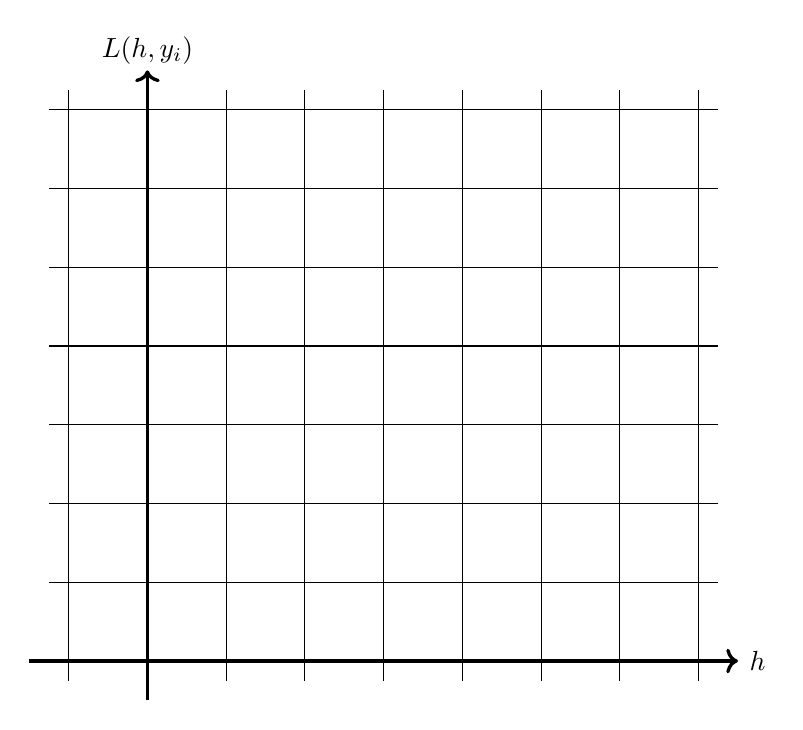
\begin{tikzpicture}[scale=1.0]
				\draw[step=1.0,black,thin] (-1.25,-0.25) grid (7.25, 7.25);
				\draw[->, very thick] (-1.5, 0) -- (7.5,0);
				\node at (7.75, 0) {$h$};
				\draw[->, very thick] (0, -0.5) -- (0,7.5);
				\node at (0, 7.75) {$L(h, y_i)$};
			\end{tikzpicture}
		\end{center}
		
		\begin{soln}
			\begin{center}
				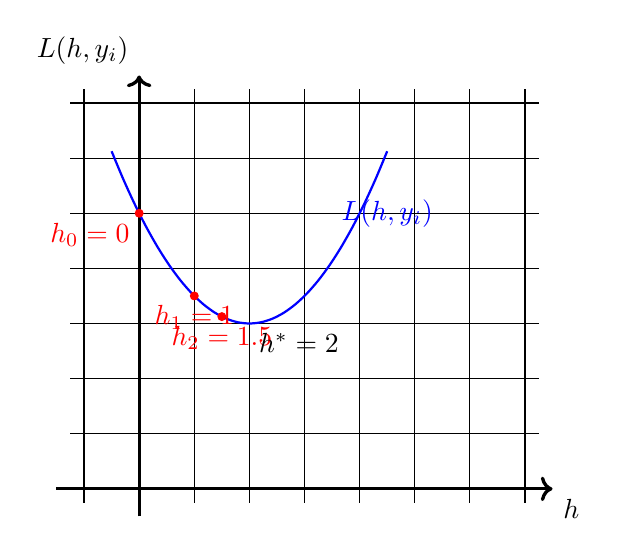
\begin{tikzpicture}[scale=0.7]
					% Draw axes
					\draw[step=1.0,black,thin] (-1.25,-0.25) grid (7.25, 7.25);
					
					\draw[->, very thick] (-1.5, 0) -- (7.5,0) node[below right] {$h$};
					\draw[->, very thick] (0, -0.5) -- (0,7.5) node[above left] {$L(h, y_i)$};
					            
					% Plot the function L(h, y_i)
					\draw[domain=-0.5:4.5, smooth, thick, blue] 
					plot (\x, {0.5*(\x-2)*(\x-2) + 3});
					\node[blue] at (4.5, 5) {$L(h, y_i)$};
					            
					% Mark h_0, h_1, h_2
					\filldraw[red] (0,5) circle (2pt) node[below left] {$h_0 = 0$};
					\filldraw[red] (1,3.5) circle (2pt) node[below] {$h_1 = 1$};
					\filldraw[red] (1.5,3.125) circle (2pt) node[below] {$h_2 = 1.5$};
					            
					% Mark optimal h*
					\draw[dashed] (2,0) -- (2,3) node[below right] {$h^* = 2$};
				\end{tikzpicture}
			\end{center}
			    
			The graph above shows:
			\begin{itemize}
				\item The loss function \(L(h, y_i) = \frac{1}{2}(h - 2)^2 + 3\) as a blue curve.
				\item The initial point \(h_0 = 0\), the first update \(h_1 = 1\), and the second update \(h_2 = 1.5\) marked as red points.
				\item The optimal height \(h^\ast = 2\) shown as a dashed vertical line.
			\end{itemize}
		\end{soln}
		
		\begin{subprob}\avo{3}
			Determine whether the gradient descent algorithm will converge to the minimum of the loss function \(L(h, y_i)\). \textit{Explain your reasoning.}
		\end{subprob}
		
		\begin{responsebox}{2in}
			The loss function \(L(h, y_i) = \frac{1}{2}(h - y_i)^2 + 3\) is a convex function because it is a quadratic function of \(h\) with a positive second derivative:
			\[
				\frac{\partial^2 L}{\partial h^2} = 1 > 0
			\]
			
			Gradient descent will converge to the minimum of a convex function if the learning rate \(\eta\) is small enough, which is the case here.
		\end{responsebox}
		
	\end{prob}
	
\end{probset}


\newpage

\begin{probset}
	
	\begin{prob}[(12 points)] %Probability
		A sample space $S$ is partitioned by three disjoint non-empty events $E_1 \cup E_2 \cup E_3=S$. Let $A \subset S$ be an event and assume you are given the following probabilities:
		\[
			P(E_1),\hspace{.1in}P(E_2),\hspace{.1in}P(A \vert E_2),\hspace{.1in}P(A \vert E_3),\hspace{.1in}\text{ and }P(A \cap E_1).
		\]
		$\bar{A}$ denotes the complement of A. 
		
		\begin{subprobset}
			\begin{subprob}\avo{5}
				Show that the probability $P(E_1 \vert \bar{A})$ can be calculated using the above terms (i.e., no probability terms are missing in order to make this calculation).
				
				\begin{responsebox}{3.5in}
					True.
					\[P(E_1 \vert \bar{A}) =  \frac{P(\bar{A} \cap E_1)}{P(\bar{A})} \]
					For the numerator
					\[P(\bar{A} \cap E_1) = P(\bar{A} \vert E_1)  * P( E_1) \]
					which we can calculate as
					\[P(\bar{A} \vert E_1) = 1-P(A \vert E_1) \]
					\[P(A \vert E_1) = \frac{P(A \cap E_1)}{P(E_1)}\]
					Therefore $P(\bar{A} \cap E_1)  = P(E_1)-P(A \cap E_1)$.
					For the denominator we use the complement
					\[P(\bar{A}) = 1-P(A) \]

                    Using the law of total probability:
					\[P(A) = P(A \vert E_1) P(E_1) +  P(A \vert E_2) P(E_2) + P(A \vert E_3) P(E_3) \]
					which we can calculate using
					\[P(E_3)=1-P(E_2)-P(E_1)\]
					
				\end{responsebox}
			\end{subprob}

            \textit{For parts \textbf{(b)}, \textbf{(c)}, and \textbf{(d)}, you do not need to show your work for full credit, but partial credit may be awarded for supporting calculations and reasoning.}
			
			\begin{subprob}\avo{3}
				For the following statements, circle either \textbf{TRUE} or \textbf{FALSE} to indicate whether the equation is correct.
				
				\textbf{(i)} $P(\bar{E_1} \vert A) =  P(E_2 \vert A) + P(E_3 \vert A)$ \hfill
				\begin{tabular}{cc}
					$\bigcirc$ TRUE & \hspace{.25in}$\bigcirc$ FALSE 
				\end{tabular}
				
				\begin{responsebox}{1in}
					TRUE - $P(\bar{E_1} \vert A) = 1 - P({E_1} \vert A) =  P(E_2 \vert A) + P(E_3 \vert A)$.
				\end{responsebox}
				
				\newpage
				\textbf{(ii)} $P(\bar{A} \vert E_1) = 1 - P(\bar{E}_1 \vert \bar{A})$ \hfill
				\begin{tabular}{cc}
					$\bigcirc$ TRUE & \hspace{.25in}$\bigcirc$ FALSE 
				\end{tabular}
				
				\begin{responsebox}{1in}
					FALSE: $P(\bar{A} \vert E_1) = 1- P({A} \vert E_1) \neq 1 - P(\bar{E}_1 \vert \bar{A})$
				\end{responsebox}
				
				\textbf{(iii)} $P(\bar{E_1} \vert A) = 1 - P(\bar{E}_1 \vert \bar{A})$ \hfill
				\begin{tabular}{cc}
					$\bigcirc$ TRUE & \hspace{.25in}$\bigcirc$ FALSE 
				\end{tabular}
				    
				\begin{responsebox}{1in}
					FALSE: $P(\bar{E_1} \vert A) = 1 - P({E}_1 \vert {A}) \neq 1 - P(\bar{E}_1 \vert \bar{A})$
				\end{responsebox}
				
			\end{subprob}
			
			% For parts \textbf{(c)} and \textbf{(d)}, fill in the circle to indicate which statement is \textbf{true}.
			
			\begin{subprob}\avo{2}
				Which of the following statements concerning $E_1,E_2,E_3$ are true? \textit{Only one statement is true.}
				
				\begin{tabular}{ll}
					$\bigcirc$ $P(\overline{E_1} \cap \overline{E_2}) = 0$  & $\bigcirc$ $P(\overline{E_1} \cup \overline{E_2}) \neq 0$ \\
					$\bigcirc$ $E1$, $E_2$ and $E_3$ are independent events & \hfill$\bigcirc$ $P(E_1 \cup E_3) = 1$                    
				\end{tabular}
				
				% \begin{enumerate}
				% \item $P(\overline{E_1} \cap \overline{E_2}) = 0$ %no \overline{E_1} \cap \overline{E_2} = E_3
				% \item $P(\overline{E_1} \cup \overline{E_2}) \neq 0$ %yes \overline{E_1} \cap \overline{E_2} = S
				% \item $E1$, $E_2$ and $E_3$ are independent events. %no
				% \item $P(E_1 \cup E_3) = 1$ %no
				% \end{enumerate}
				
				\begin{responsebox}{3in}
                
					Correct: $ \overline{E_1} \cup \overline{E_2} = (E_2 \cup E_3) \cup (E_1 \cup E_3) = S \rightarrow P(\overline{E_1} \cup \overline{E_2}) = 1$.
					
					Incorrect: $P(\overline{E_1} \cap \overline{E_2}) = P((E_2 \cup E3) \cap (E_1 \cup E_3)) = P(E_3) \neq 0$
					
					Incorrect: $P(E_1 \cup E_3) = 1 - P(E_2) < 1$ since $E_2$ is non empty. 
					
					Incorrect $E1$, $E_2$ and $E_3$ are not independent since $P(E_1,E_2,E_3) = P(E_1 \cap E_2 \cap E_3) = P(\emptyset)= 0 \neq P(E_1)P(E_2)P(E_3)>0$ 
				\end{responsebox}
				
			\end{subprob}
			
	%		\newpage
			\begin{subprob}\avo{2}
				If the event $E_1$ is fully contained within event $A$, i.e., every outcome in $E_1$ is also an outcome in $A$, we write that $E_1 \subseteq A$. Which if the following statements is true? \textit{Only one statement is true.}
				
				\begin{tabular}{l}
					$\bigcirc$ If $E_1 \subseteq A$, then $P(E_1)\leq P(A)$.                    \\
					$\bigcirc$ If $P(E_1)\leq P(A)$, then $E_1 \subseteq A$.                    \\
					$\bigcirc$ If $E_1 \subseteq A$, then $P(E_1 \cap A)\leq P(E_2)$.           \\
					$\bigcirc$ If $E_1 \subseteq A$, then $E_1$ and $A$ are independent events. \\
					$\bigcirc$ If $E_1 \subseteq A$, then $E_3$ and $A$ are independent events. 
				\end{tabular}
				
				% \begin{enumerate}
				% \item If $E_1 \subseteq A$, then $P(E_1)\leq P(A)$. %true
				% \item If $P(E_1)\leq P(A)$, then $E_1 \subseteq A$. %false
				% \item If $E_1 \subseteq A$, then $P(E_1 \cap A)\leq P(E_2)$. %false
				% %\item If $E_1 \subseteq A$, then $P(E_1 \cap A) = P(E_1)$. %true
				% \item If $E_1 \subseteq A$, then $E_1$ and $A$ are independent events. %false
				% \item If $E_1 \subseteq A$, then $E_3$ and $A$ are independent events. %false
				% \end{enumerate}
				
				\begin{responsebox}{2in}
					%Alternate versions included either 1 or 4, both are true.
					
					Correct: $P(E_1) = \sum_{s \in E_1} p(s)$ and $P(A) = \sum_{s \in A} p(s)$.
					Since $\forall s \in E_1: s \in A$, then $P(E_1)\leq P(A)$.
					
					%Correct: Since $\forall s \in E_1: s \in A$, then $E_1 \cap A =  E_1$, therefore $P(E_1 \cap A) = P(E_1)$.

                    The converse is not true:
                    $P(E_1)\leq P(A)$ can be true without  $E_1 \subseteq A$.   

                    When $E_1 \subseteq A$ then $P(E_1)=P(E_1 \cap A)$ however we don't know anything about the relationship between $P(E_1)$ and $P(E_2)$.

                    If $E_1 \subseteq A$ these are not independent events since $P(E_1 | A) = 1 \neq P(E_1)$.
                    
				\end{responsebox}
				 
			\end{subprob}
		\end{subprobset}
		
	\end{prob}
	
\end{probset}

\newpage

\begin{probset}
	\begin{prob}[(13 points)] %Probability
		
		Robert has a sock drawer containing exactly eight socks: one pair each of plain socks, dotted socks, striped socks, and plaid socks.
		        
		\begin{subprob}\avo{3}
			On Monday morning while getting ready, Robert selects two socks at random from the drawer. What is the probability that the socks are matching? \textit{Explain your reasoning.}
		\end{subprob}
		
		\begin{responsebox}{1in}
			There are ${8\choose 2}$ ways to pick the two socks from the drawer, of which exactly four pairs are matching. Therefore the probability is 
			\[\frac{4}{{8\choose 2}} = \frac{(4)(2)}{(8)(7)} = \frac{1}{7}.\]
		\end{responsebox}
		
		\begin{subprob}\avo{4}
			After wearing the socks on Monday he places them in a laundry basket separate from the drawer. On Tuesday morning, as Robert gets ready, he selects another two socks at random from the six remaining in the drawer. What is the probability that the socks are matching on Tuesday? \textit{Show all your calculations.}
		\end{subprob}
		
		\begin{responsebox}{3in}
			We can condition on whether the socks were matching on Monday and use this information to our advantage. Specifically,
			\begin{align*}
				\pr{\text{match on Tues.}} & = \pr{\text{match on Tues.}|\text{match on Mon.}}\pr{\text{match on Mon.}}              \\
				                           & +  \pr{\text{match on Tues.}|\text{don't match on Mon.}}\pr{\text{don't match on Mon.}} \\
				                           & = \pr{\text{match on Tues.}|\text{match on Mon.}}\frac{1}{7}                            \\
				                           & + \pr{\text{match on Tues.}|\text{don't match on Mon.}}(1 - \frac{1}{7})                
			\end{align*}
			If the socks were matching on Monday, there are now three pairs of matching socks in the drawer. So we have, by the same logic as before,
			\begin{align*}
				\pr{\text{match on Tues.}|\text{match on Mon.}} & = \frac{3}{{6\choose 2}} = \frac{(3)(2)}{(6)(5)} = \frac{1}{5}. 
			\end{align*}
			If the socks were not matching on Monday, there are now two pairs of matching socks plus two mismatching socks. The total number of pairs is still ${6\choose 2}$ but now only two such pairs match. Therefore,
			\begin{align}
				\pr{\text{match on Tues.}|\text{don't match on Mon.}} & = \frac{2}{{6\choose 2}} =\frac{(2)(2)}{(6)(5)} = \frac{2}{15}. 
			\end{align}
			Thus in conclusion we have
			\begin{align}
				\pr{\text{match on Tues.}} & = \frac{1}{5}\frac{1}{7} + \frac{2}{15}\frac{6}{7}. 
			\end{align}
		\end{responsebox}
		
		\newpage
		\begin{subprob}(\avo{1}$\times$6)
			On Tuesday evening Robert does laundry so that when he gets ready on Wednesday morning all of the socks are clean again. As usual he selects another two socks at random, a selection which is independent of any of his choices on Monday or Tuesday. What is the probability that he wears at least one striped sock on Monday, Tuesday, \textbf{and} Wednesday? \textit{Show all your calculations.}
		\end{subprob}
		
		\begin{responsebox}{4in}
			Based on the setup, Robert must have worn exactly one striped sock on both Monday and Tuesday, and then wore either a single striped sock or a pair of striped socks on Wednesday. By the definition of conditional probability, we have
			\begin{align*}
				\pr{\text{1 striped on Mon.}\cap \text{1 striped on Tues.}} & = \pr{\text{1 striped on Tues.} | \text{1 striped on Mon.} } \\
				                                                            & \times \pr{\text{1 striped on Mon.}}                         
			\end{align*}
			For Monday, there are ${2\choose 1}{6\choose 1} = 12$ possible pairs of socks so that exactly one is striped. Thus the probability is given by
			\begin{align*}
				\pr{\text{1 striped Mon.}} & = \frac{12}{{8\choose 2}} = \frac{(12)(2)}{(8)(7)} = \frac{3}{7}. 
			\end{align*}
			Alternatively, you could write this as 1 minus the probability of getting either no striped socks or two striped socks. For the second part, by similar logic, we have
			\begin{align*}
				\pr{\text{1 striped on Tues.} | \text{1 striped on Mon.} } & = \frac{{1\choose 1}{5\choose 1}}{{6\choose 2}} = \frac{(5)(2)}{(6)(5)} = \frac{1}{3}. 
			\end{align*}
			Therefore we have   
			\begin{align*}
				\pr{\text{1 striped on Mon.}\cap \text{1 striped on Tues.}} = \frac{3}{7}\frac{1}{3} = \frac{1}{7}. 
			\end{align*}
			For Wednesday, he can select either one or two striped socks. Earlier we counted $12$ pairs which contain exactly one striped sock, so there are $13$ which contain either one or two. Thus
			\begin{align*}
				\pr{\text{ 1 or 2 striped on Weds.}} & = \frac{13}{{8\choose 2}} = \frac{13}{28}. 
			\end{align*}
			By the independence assumption, we have
			\begin{align*}
				  & \pr{\text{1 striped on Mon.}\cap \text{1 striped on Tues.} \cap \geq\text{1 striped Weds.}} \\
				  & =  \pr{\text{1 striped on Mon.}\cap \text{1 striped on Tues.}}                              \\
				  & \times \pr{\geq\text{1 striped Weds.}}                                                      \\
				  & = \frac{13}{(7)(28)}                                                                        
			\end{align*}
		\end{responsebox}
		        
	\end{prob}
\end{probset}


\newpage

\begin{probset}
	
	%\newpage
	\begin{prob}[(11 points)] %Independence
		    
		You have 4 sets of dishes each consisting of plates (dessert and dinner), cutlery (spoon fork and knife) and cups (glass, wineglass and mug). Two sets are red and two are blue and each set has a different pattern:  dots,  solid,  stripes or flowers as in the picture below. Originally you had $4 * 8 =32$ dishes, but over the years you have lost some of your dishes so that now you only have 28. A lost dish is indicated by dish being missing in the image (for example you lost the blue flowers dessert place or the red dots mug). 
		    
		\begin{center}
			\includegraphics[width=0.75\textwidth]{prob_plates.png} 
		\end{center}
		    
		You come home and find a single item in the kitchen sick.
		
\begin{responsebox}{1.5in}
Note this question is based on Lecture 23, slides 15, 20, 21 where we have replaced a deck of cards with patterned dishes.

In both b) and c) many made the mistake of selecting disjoint events A and B such the $A \cap B = \emptyset$ (or $A \cap B|C = \emptyset$ in c) ) but $P(A),P(B)>0$.
Mutually exclusive events with non-zero probability are not independent (lecture 23, slide 13).



\end{responsebox}

        
		\begin{subprobset}
			\begin{subprob}\avo{3}
				Let $A$ be the event that the item has stripes, and let $B$
				be the event that the item is a cup (glass, wineglass or mug). Are these events independent? \textit{Explain your reasoning.}
				
				\begin{responsebox}{1.5in}
                This question is based on the deck of cards question we did in class. 
                
					No, they are not. Knowing that the item is a cup makes it
					slightly more likely that the item has stripes.
					                    
                    $$P(A)=7/28 $$
                    $$P(B)=10/28 = 5/14$$
                    $$P(A \cap B = 3/28 \neq (7*5)/(28*14)=5/56 $$
                    Therefore not independent 
                    
%Alternate version: cup and flowers is the same as cup and stripes. For cutlery and checkerboard, knowing the item is cutlery makes checkerboard slightly more likely.                     
				\end{responsebox}
			\end{subprob}
			
%			\newpage
			\begin{subprob}\avo{4}
				Regarding the identity of the item in the sink, give an example of two events $A$ and $B$ which are \emph{independent}. Prove that they are independent. \textit{To receive full credit, your events should not have probabilities equal to zero or to one.}
				
				\begin{responsebox}{2in}

                    There were multiple correct options here.

                    One strategy is based on noticing that in every row there are 7 dishes.
                    Therefore for any dish for which we have all 4 patterns (dinner plate, spoon, knife, wine glass) you can select event A to be a pattern (for example dots) and B to be one of the dishes for which we have the full set (for example spoon).
                    Then 
                    $$P(A) = \frac{7}{28}=\frac{1}{4}$$
                    $$P(B) = \frac{4}{28}=\frac{1}{7}$$
                    $$P(A \cap B) = \frac{1}{28} = \frac{1}{7} \cdot \frac{1}{4}$$

                    Also
                    $$P(B|A) = \frac{1}{7}=P(B)$$

                    This can also be done for either the red or blue color (instead of a single pattern), for example:  
					Let A be the event that the item is red and let B be the event that the item is a spoon. There are 14 red dishes: $P(A)=\frac{14}{28}=\frac{1}{2}$ and there are 4 spoons: $P(B)=\frac{4}{28}=\frac{1}{7} $. There are 2 red spoons: $P(A,B) =\frac{2}{28}=\frac{1}{14}$. 
					\[ P(A,B)= \frac{1}{14} =\frac{1}{7}* \frac{1}{2} =P(B)*P(A) \]
				\end{responsebox}

                    
                
			\end{subprob}
			
			\begin{subprob}\avo{4}
				Regarding the identity of the item in the sink, give an example of three events $A$, $B$, and $C$ such that $A$ and $B$ are \emph{conditionally independent} given $C$. Prove that they are conditionally independent. \textit{To receive full credit, your events should not have probabilities equal to zero or to one.}
				
			\begin{responsebox}{2in}
                As in b) there are many correct solutions here (some of you were very creative).
                
                One strategy here is to consider the events in a) which weren't independent and see if we can condition it on event C, so that they are.
                Let  $A$ be the event that the item has stripes, and let $B$  be the event that the item is a cup (glass, wineglass or mug). 
                Notice if we set $C$ to be the event that the item is blue,
                none of the blue cups are missing.

                Then, there are 3 blue striped cups: $P(A\cap B|C)= \frac{3}{14}$. There are seven blue striped dishes $P(A|C)=\frac{7}{14}=\frac{1}{2}$ and there are 6 blue cups: $P(B|C)=\frac{6}{14}=\frac{3}{7}$.
					\[ P(A\cap B|C)= \frac{3}{14} =\frac{1}{2}*\frac{3}{7}=P(A|C)*P(B|C)  \]

                Some other popular answers:
                
                A = dots, B = plates, C= red   (this also works for A = solid)

                $$P(A|C) = \frac{7}{14}=\frac{1}{2}$$
                $$P(B|C) = \frac{4}{14}=\frac{2}{7}$$
                $$P(A \cap B|C) = \frac{2}{14}$$
                
                 A = stripe, B = knife, C= blue
                 (this also works for A = flowers, and/or B = spoon)
                $$P(A|C) = \frac{7}{14}=\frac{1}{2}$$
                $$P(B|C) = \frac{2}{14}=\frac{1}{7}$$
                $$P(A \cap B|C) = \frac{1}{14}$$
                
                
                We did accept cases (with some deduction) where 
$$P(A |C) =0$$
$$P(B|C)>0$$
$$P(A \cap B |C) =0$$

or 
$$P(A |C) =1$$
$$P(B|C)>0$$
$$P(A \cap B |C) = P(B|C)$$
                
                
				\end{responsebox}
			\end{subprob}
		\end{subprobset}
		        
		        
		
	\end{prob}
	
\end{probset}

\newpage


\begin{probset}
	% %%% Naive Bayes Classifier
	% \section*{Naive Bayes Classifier}
	
	\begin{prob}[(8 points)] %Naive Bayes 
		You work for Amazon and are implementing a book genre classifier to determine whether a book is science fiction (sci-fi), romance or thriller based on details of the plot. 
		You have a dataset of 18 books and 4 features  \{``Happy conclusion",``Spaceships",``Murder investigation",``Sidekick" \} to train a Na\"ive Bayes classifier.
		       
		\begin{center}
			\begin{tabular}{c|c|cccc}
				Book \# & Genre    & Murder & Sidekick & Happy & Spaceships \\
				1       & sci-fi   & No     & \yes     & \yes  & \yes       \\
				2       & sci-fi   & No     & \yes     & \yes  & No         \\
				3       & sci-fi   & No     & No       & \yes  & \yes       \\
				4       & sci-fi   & No     & \yes     & No    & \yes       \\
				5       & sci-fi   & \yes   & \yes     & No    & \yes       \\
				6       & sci-fi   & No     & \yes     & \yes  & \yes       \\
				7       & sci-fi   & No     & \yes     & \yes  & \yes       \\
				8       & sci-fi   & No     & No       & No    & \yes       \\
				9       & sci-fi   & No     & \yes     & No    & \yes       \\
				10      & sci-fi   & \yes   & \yes     & No    & \yes       \\ \hline
				11      & romance  & No     & No       & \yes  & \yes       \\
				12      & romance  & No     & \yes     & \yes  & No         \\
				13      & romance  & No     & \yes     & \yes  & No         \\
				14      & romance  & \yes   & No     & \yes  & No         \\
				15      & romance  & No     & No       & \yes  & No         \\
				16      & romance  & \yes   & \yes     & \yes  & No         \\ \hline
				17      & thriller & \yes   & \yes     & No    & No         \\ 
				18      & thriller & \yes   & No       & \yes  & No         \\
				19      & thriller & \yes   & \yes     & No    & \yes       \\ 
				20      & thriller & \yes   & \yes     & \yes  & No         \\
			\end{tabular}
		\end{center}
		
		\begin{subprob}(\avo{1}$\times$8)
			A new book has been released which has `Happy conclusion", ``sidekick" but not  ``Spaceships" or ``murder investigation". Is this book a sci-fi, thriller or romance?  Use the Naive Bayes Classifier without smoothing. Be sure to clearly state your prediction as one of the three genres. \textit{Show all your calculations.}
		\end{subprob}
		
		\begin{responsebox}{2in}
			
		\end{responsebox}
		
		
		\begin{responsebox}{8in}
			We estimate the following probabilities from the table:
			\begin{align*}
				P(\text{Happy} \given \text{romance})         & = 6/6=1     \\
				P(\text{sidekick} \given \text{romance})      & = 3/6=1/2   \\
				P(\text{No Murder} \given \text{romance})     & = 4/6=2/3   \\
				P(\text{No Spaceships} \given \text{romance}) & = 5/6       \\
				P(\text{romance})                             & = 6/20=3/10 \\[1em]
				P(\text{Happy} \given \text{sci-fi})          & = 5/10      \\
				P(\text{sidekick} \given \text{sci-fi})       & = 8/10=4/5  \\
				P(\text{No Murder} \given \text{sci-fi})      & = 8/10=4/5  \\
				P(\text{No Spaceships} \given \text{sci-fi})  & = 1/10      \\
				P(\text{sci-fi})                              & = 10/20=1/2 \\[1em]
				P(\text{No Murder} \given \text{thriller})    & = 0/4       
			\end{align*}
			
			Therefore:
			\begin{align*}
				  & P(\text{romance} \given \text{Happy,Sidekick, Murder, No Spaceships}) \\
				  &                                                                       
				\qquad 
				\propto
				P(\text{Happy}\given\text{romance})\\
				  & \qquad \qquad                                                         
				\times
				P(\text{sidekick}\given\text{romance})\\
				  & \qquad \qquad                                                         
				\times
				P(\text{No Murder}\given\text{romance})\\
				  & \qquad \qquad                                                         
				\times
				P(\text{No Spaceships}\given\text{romance})\\
				  & \qquad \qquad                                                         
				\times
				P(\text{romance})\\
				  & =                                                                     
				1 \cdot \frac{1}{2}  \cdot \frac{2}{3} \cdot \frac{5}{6} \cdot \frac{3}{10}  
				= \frac{1}{2}   \cdot \frac{1}{3} \cdot \frac{1}{2}  =
				\frac{1}{12}
			\end{align*}
			
			\begin{align*}
				  & P(\text{sci-fi} \given \text{Happy,Sidekick, Murder, No Spaceships}) \\
				  &                                                                      
				\qquad 
				\propto
				P(\text{Happy}\given\text{sci-fi})\\
				  & \qquad \qquad                                                        
				\times
				P(\text{sidekick}\given\text{sci-fi})\\
				  & \qquad \qquad                                                        
				\times
				P(\text{Murder}\given\text{sci-fi})\\
				  & \qquad \qquad                                                        
				\times
				P(\text{No Spaceships}\given\text{sci-fi})\\
				  & \qquad \qquad                                                        
				\times
				P(\text{sci-fi})\\
				  & =                                                                    
				\frac{5}{10} \cdot \frac{4}{5} \cdot \frac{4}{5} \cdot \frac{1}{10}
				\cdot \frac{1}{2}
				=
				\frac{4}{5} \cdot \frac{1}{5} \cdot \frac{1}{10} 
				=
				\frac{2}{125}
			\end{align*}
			
			\begin{align*}
				  & P(\text{thriller} \given \text{Happy,Sidekick, Murder, No Spaceships}) \\
				  &                                                                        
				\qquad 
				\propto
				P(\text{Happy}\given\text{thriller})\\
				  & \qquad \qquad                                                          
				\times
				P(\text{sidekick}\given\text{thriller})\\
				  & \qquad \qquad                                                          
				\times
				P(\text{No Murder}\given\text{thriller})\\
				  & \qquad \qquad                                                          
				\times
				P(\text{No Spaceships}\given\text{thriller})\\
				  & \qquad \qquad                                                          
				\times
				P(\text{thriller})\\
				  & =                                                                      
				0
			\end{align*}
			
			Since the first probability is the largest, our prediction is that the book was romance.
		\end{responsebox}
	\end{prob}
	
\end{probset}


\newpage


\end{document}